\chapter*{Dodatak: Prikaz aktivnosti grupe}
		
		\section*{Dnevnik sastajanja}
		
		\begin{packed_enum}
			\item  sastanak
			
			\item[] \begin{packed_item}
				\item Datum: 7. listopada 2020.
				\item Prisustvovali: Mateja Iveta, Dora Horvat, Vedran Hernaus, Lea Brzica, Matija Holik, Denis Đurašinović , Dora Bortas
				\item Teme sastanka:
				\begin{packed_item}
					\item  Upoznavanje članova tima
					\item  Dogovor o tehnologijama. Dogovoreno: Postgres - Spring - React
					\item Dogovor o prijedlogu drugog projektnog zadatka
				\end{packed_item}
			\end{packed_item}
			
			\item  sastanak
			\item[] \begin{packed_item}
				\item Datum: 15. listopada 2020.
				\item Prisustvovali:  Mateja Iveta, Dora Horvat, Vedran Hernaus, Lea Brzica, Matija Holik, Denis Đurašinović , Dora Bortas
				\item Teme sastanka:
				\begin{packed_item}
					\item  Razgovor o funkcionalnim zahtjevima sustava i arhitekturi
					
				\end{packed_item}
			\end{packed_item}
			\item  sastanak
			
			\item[] \begin{packed_item}
				\item Datum: 19. listopada 2020.
				\item Prisustvovali: Mateja Iveta, Dora Horvat, Vedran Hernaus, Lea Brzica, Matija Holik, Denis Đurašinović , Dora Bortas
				\item Teme sastanka:
				\begin{packed_item}
					\item Definiranje organizacije baze podataka
					\item Dogovor o raspodjeli poslova
				\end{packed_item}
			\end{packed_item}
		
			
				\item  sastanak
				
				\item[] \begin{packed_item}
					\item Datum: 22. listopada 2020.
					\item Prisustvovali: Mateja Iveta, Dora Horvat, Vedran Hernaus, Lea Brzica, Matija Holik, Denis Đurašinović , Ivana Cepetić, Luka Martić
					\item Teme sastanka:
					\begin{packed_item}
						\item Razgovor o optimalnoj organizaciji baze podataka
					\end{packed_item}
				\end{packed_item}
				\item  sastanak
			
			\item[] \begin{packed_item}
				\item Datum: 29. listopada 2020.
				\item Prisustvovali: Mateja Iveta, Dora Horvat, Vedran Hernaus, Lea Brzica, Matija Holik, Denis Đurašinović , Dora Bortas
				\item Teme sastanka:
				\begin{packed_item}
					\item Podjela uloga za kreiranje baze, izradu kontrolera, servisa i repozitorija, dokumentacije i logina i registgracije
				\end{packed_item}
			\end{packed_item}
		 \item sastanak
		\item[] \begin{packed_item}
			\item Datum: 4. studenoga 2020.
			\item Prisustvovali:  Dora Horvat, Dora Bortas, Ivana Cepetić, Luka Martić
			\item Teme sastanka:
			\begin{packed_item}
				\item Razgovor o trenutnom napretku dokumentacije
				
			\end{packed_item}
		\end{packed_item}
	\item sastanak
		\item[] \begin{packed_item}
			\item Datum: 6. studenoga 2020.
			\item Prisustvovali: Mateja Iveta, Dora Horvat, Vedran Hernaus, Lea Brzica, Matija Holik, Denis Đurašinović , Dora Bortas
			\item Teme sastanka:
			\begin{packed_item}
				\item Diskusija o trenutnom napretku projekta
				\item Podjela poslova koji se moraju obaviti do prve predaje projekta
			\end{packed_item}
		\end{packed_item}
			\item sastanak
			\item[] \begin{packed_item}
				\item Datum: 12. studenoga 2020.
				\item Prisustvovali: Mateja Iveta, Dora Horvat, Vedran Hernaus, Lea Brzica, Matija Holik, Denis Đurašinović , Dora Bortas, Ivana Cepetić, Luka Martić, Hrvoje Šimić
				\item Teme sastanka:
				\begin{packed_item}
					\item Pregled generičkih funkcionalnosti aplikacije prije prve predaje
				\end{packed_item}
			\end{packed_item}
			%
			
		\end{packed_enum}
		
		\eject
		\section*{Tablica aktivnosti}
		
			\textbf{\textit{Kontinuirano osvježavanje}}\\
			
			 \textit{Napomena: Doprinose u aktivnostima treba navesti u satima po članovima grupe po aktivnosti.}
					
						
			
			\begin{longtabu} to \textwidth {|X[7, l]|X[1, c]|X[1, c]|X[1, c]|X[1, c]|X[1, c]|X[1, c]|X[1, c]|}
								
				\cline{2-8} \multicolumn{1}{c|}{\textbf{}} &     \multicolumn{1}{c|}{\rotatebox{90}{\textbf{ Mateja Iveta }}} & \multicolumn{1}{c|}{\rotatebox{90}{\textbf{Dora Bortas }}} &	\multicolumn{1}{c|}{\rotatebox{90}{\textbf{Dora Horvat }}} &	\multicolumn{1}{c|}{\rotatebox{90}{\textbf{Lea Brzica }}} &
				\multicolumn{1}{c|}{\rotatebox{90}{\textbf{Vedran Hernaus }}} &
				\multicolumn{1}{c|}{\rotatebox{90}{\textbf{Matija Holik }}} &	\multicolumn{1}{c|}{\rotatebox{90}{\textbf{Denis Đurašinović }}} \\ \hline 
				\endfirsthead
				
			
				\cline{2-8} \multicolumn{1}{c|}{\textbf{}} &     \multicolumn{1}{c|}{\rotatebox{90}{\textbf{Mateja Iveta}}} & \multicolumn{1}{c|}{\rotatebox{90}{\textbf{Dora Bortas }}} &	\multicolumn{1}{c|}{\rotatebox{90}{\textbf{Dora Horvat }}} &
				\multicolumn{1}{c|}{\rotatebox{90}{\textbf{Lea Brzica }}} &	\multicolumn{1}{c|}{\rotatebox{90}{\textbf{Vedran Hernaus }}} &
				\multicolumn{1}{c|}{\rotatebox{90}{\textbf{Matija Holik }}} &	\multicolumn{1}{c|}{\rotatebox{90}{\textbf{Denis Đurašinović }}} \\ \hline 
				\endhead
				
				
				\endfoot
							
				 
				\endlastfoot
				
				Upravljanje projektom 		&  &  & 1 &  &  &  & \\ \hline
				Opis projektnog zadatka 	&  &  & 6 &  &  &  & \\ \hline
				
				Funkcionalni zahtjevi       &  & 3 &  &  &  &  &  \\ \hline
				Opis pojedinih obrazaca 	&  & 5 &  &  &  &  &  \\ \hline
				Dijagram obrazaca 			&  & 3 &  &  &  &  &  \\ \hline
				Sekvencijski dijagrami 		&  & 3 &  &  &  &  &  \\ \hline
				Opis ostalih zahtjeva 		&  & 1 &  &  &  &  &  \\ \hline

				Arhitektura i dizajn sustava&  & 1 &  &  &  &  &  \\ \hline
				Baza podataka				&  &  & 10 &  &  &  &   \\ \hline
				Dijagram razreda 			&  & 5 &  &  &  &  &   \\ \hline
				Dijagram stanja				&  &  &  &  &  &  &  \\ \hline
				Dijagram aktivnosti 		&  &  &  &  &  &  &  \\ \hline
				Dijagram komponenti			&  &  &  &  &  &  &  \\ \hline
				Korištene tehnologije i alati 		&  &  &  &  &  &  &  \\ \hline
				Ispitivanje programskog rješenja 	&  &  &  &  &  &  &  \\ \hline
				Dijagram razmještaja			&  &  &  &  &  &  &  \\ \hline
				Upute za puštanje u pogon 		&  &  &  &  &  &  &  \\ \hline 
				Dnevnik sastajanja 			&  &  &  &  &  &  &  \\ \hline
				Zaključak i budući rad 		&  &  &  &  &  &  &  \\  \hline
				Popis literature 			&  &  &  &  &  &  &  \\  \hline
				&  &  &  &  &  &  &  \\ \hline \hline
				Izrada frontenda 		 	& 10 &  &  & 25 & 20 &  &  \\ \hline
				Izrada backenda 		 	& 25 &  &  &  & 4 & 30 & 4 \\ \hline 
				Sigurnost					&  &  &  &  &  & 10 & \\ \hline 
				Spajanje na bazu 		 	&25  &  &  &  &  &  & \\ \hline 
				Modeliranje baze 			&  &  &  &  &  &  & 20 \\ \hline
				Puštanje u pogon		 	&10  &  &  &  &  &  &  \\  \hline
				 						
				
				
			\end{longtabu}

			\section*{Dijagrami pregleda promjena}
		
		\begin{figure}[H]
			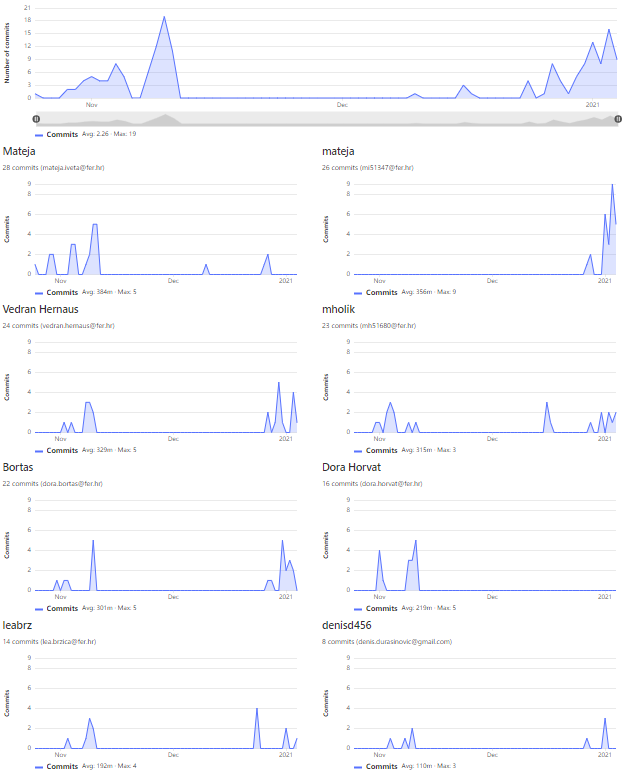
\includegraphics[scale=0.9]{slike/repository.png} %veličina slike u odnosu na originalnu datoteku i pozicija slike
			\centering
			\caption{Dijagrami aktivnosti na master grani}
			\label{fig:aktivnost}
		\end{figure}
					
					
		\eject
	
	
